
\begin{enumerate}[label=\thesection.\arabic*.,ref=\thesection.\theenumi]
\numberwithin{equation}{enumi}
\item Question-The open loop transfer function of a unity feedback system is given by
\begin{align*}
 G(s)=\frac{\pi e^{-0.25s}}{s}
\end{align*}
in G(s) plane,the Nyquist plot of G(s) passes through the negative real axis at the point
\\*(A)(-0.5,j0)  (B)(-0.75,j0)  (C)(-1.25,j0)  (D)(-1.5,j0)


 

\begin{frame}{SOLUTION}
\begin{itemize}


\begin{equation*}

G(s)=\frac{\pi e^{-0.25s}}{s}

\end{equation*}

 Nyquist plot cuts the negative real
Axis at $\omega$ = phase cross over frequency,at phase cross over frequency the phase of nyquist plot becomes -$\pi$ radians.
\\
\newline substitute s=j$\omega$.
\\
\newline \(G(j\omega)=\frac{\pi}{\omega}(-\sin{0.25$\omega$}-j\cos{0.25$\omega$})\).
\\
\newline \angle G(j$\omega$)=-$\pi$/2 -0.25$\omega$.
\\
\newline\angle G(j$\omega$)|$_{\omega=\omega_{pc}}$=-$\pi$ radians
\\
\newline by solving for $\omega$ we get $\omega_{pc}=2\pi$.
\\
\newline magnitude at any point is X=$|G(j\omega)|$=$\frac{\pi}{\omega}$.
\\
\newline substituting $\omega=2\pi$ in magnitude equation we get X=0.5.
\\
\newline hence it intersects at (-0.5,0j) so answer is A.
\\

\end{itemize}
\end{frame}
\begin{frame}{plot verification}
\newline we can verify with the following plot that it intersects at (-0.5,0j)
\begin{figure}
  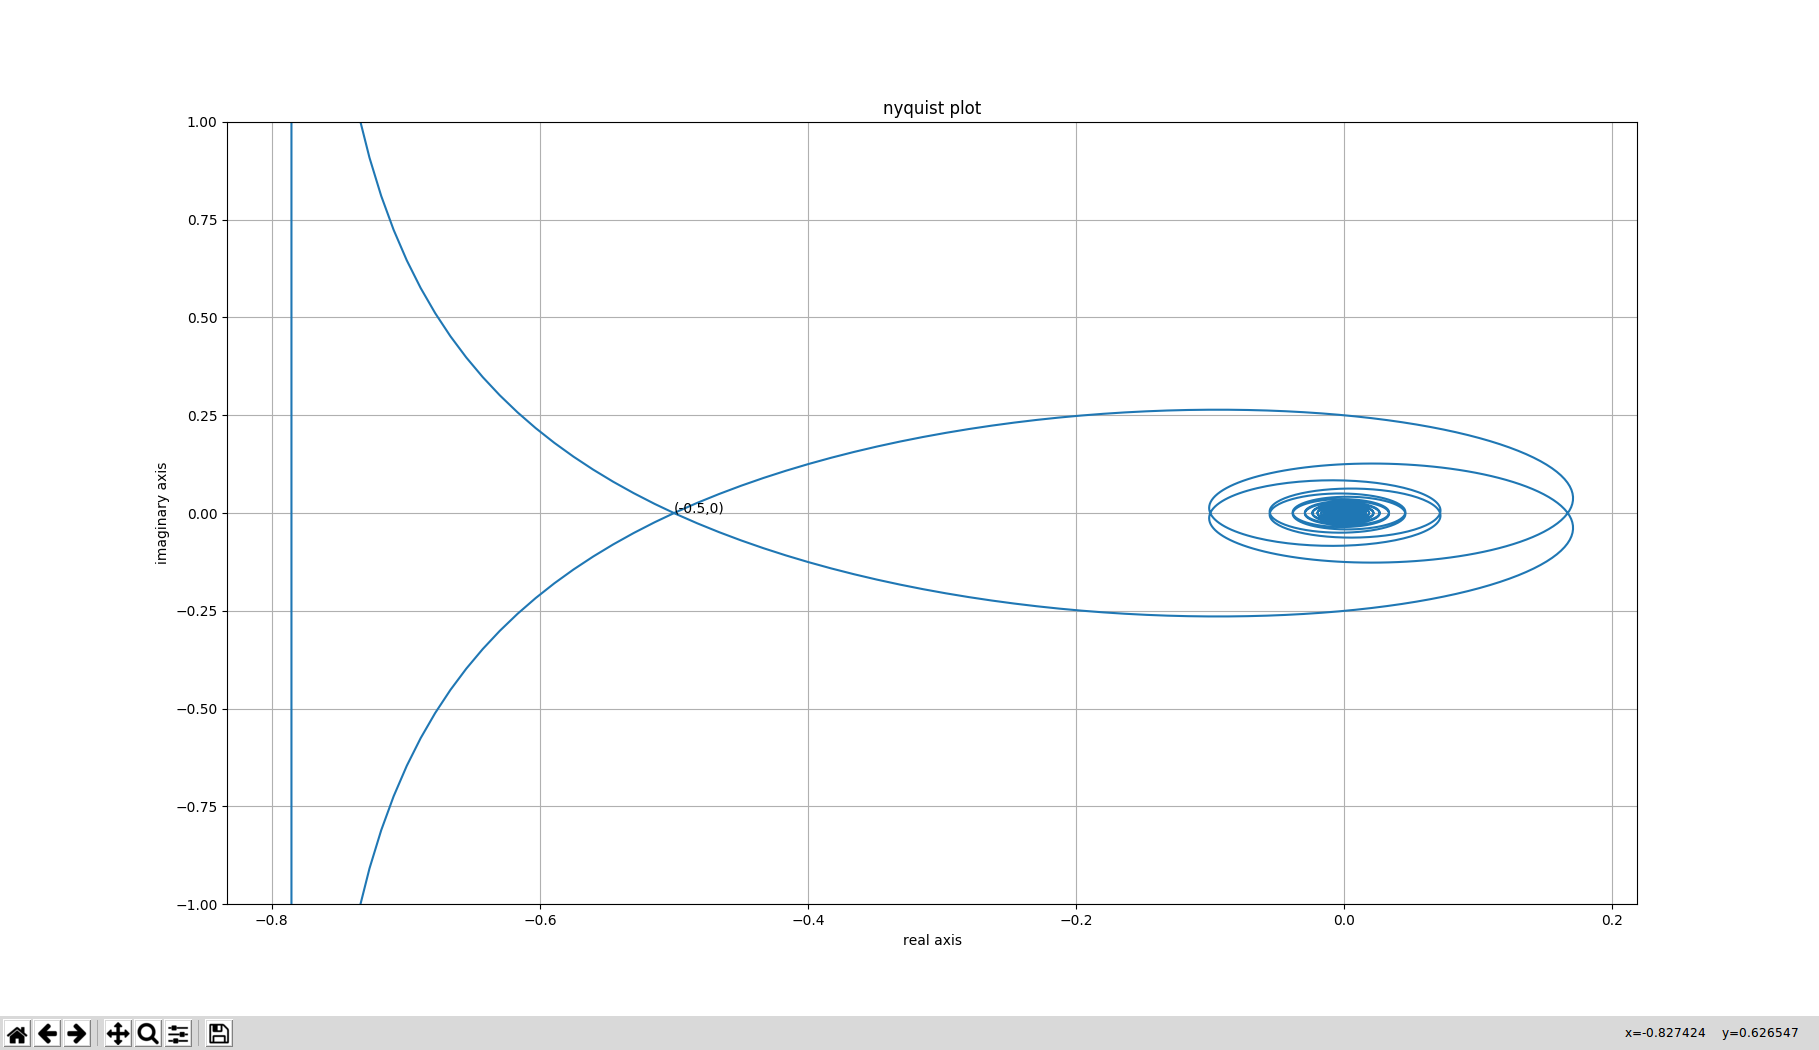
\includegraphics[width=\linewidth]{nyquist.eps}
  \caption{Nyquist plot}
  \label{fig:Nyquist plot}
\end{figure}
\begin{itemize}
\end{itemize}
\end{frame}

\end{enumerate}
